

\begin{frame}{The Gender Incidence of the Consolidation}
\hypertarget{src:gender}{}
\small
A net effect can hide an offsetting transfer, so we open the consolidation itself. It moves vote from the runner-up's slot to the winner's; splitting both slots by the office-seeker's gender asks who pays and who collects. The split is unconditional: the components sum back exactly to the totals on the previous frames, with the same $N$ and nothing conditioned on who placed where \hyperlink{app:gender}{\beamergotobutton{construct \& full tables}}.
\smallskip
\begin{center}
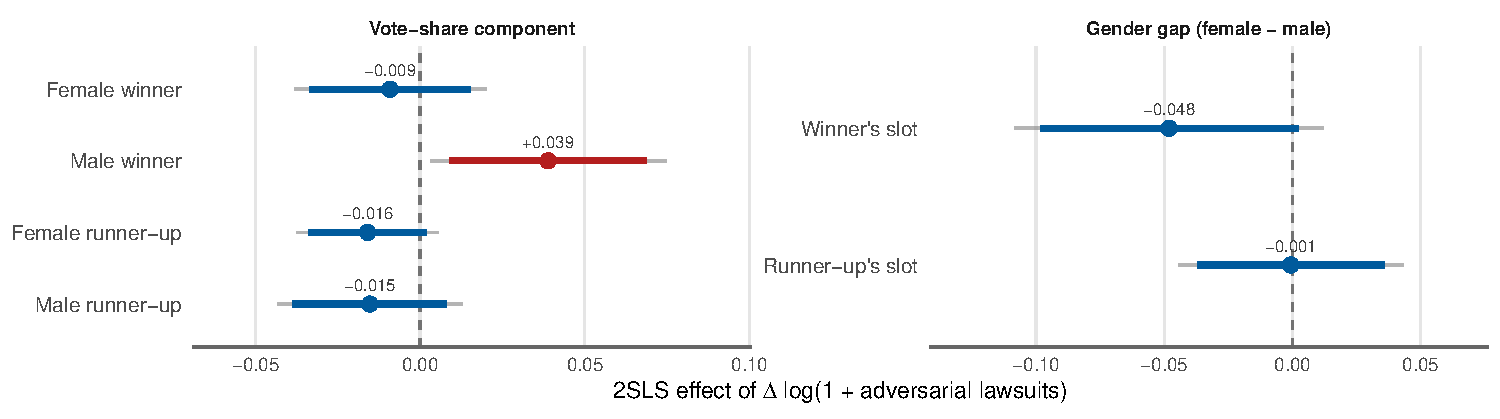
\includegraphics[width=\linewidth,height=0.32\textheight,keepaspectratio]{../figures/gender_consolidation_coefplot.pdf}
\end{center}
\smallskip
\takeaway{The cost is gender-neutral, while the gain may not be. The runner-up's loss splits evenly (female $\FemRUSharePerSDSigned$~pp, male $\MaleRUSharePerSDSigned$~pp) and that slot's gap is a precisely estimated zero ($\RUGapCoef$, $p=\RUGapP$) rather than an inconclusive one. The gain lands on male front-runners ($\MaleWinSharePerSDSigned$~pp, $p=\MaleWinShareP$) while the female winner's share is flat ($p=\FemWinShareP$), but that slot's differential test is $\WinGapPerSDSigned$~pp, $p=\WinGapP$: \negt{suggestive, not established}. Net, women's share of the top two drifts down $\FemTopTwoPerSDSigned$~pp ($p=\FemTopTwoP$).}
\smallskip
\scriptsize\ns{This is the incidence the demographic profile of the top two implies: if winner and runner-up are near-twins \hyperlink{src:favored}{\beamergotobutton{who it favors}}, widening the margin between them should be gender-blind on the losing side, and it is. Exploratory, outside the declared family, raw $p$ \hyperlink{app:multiplicity}{\beamergotobutton{multiplicity}}.}
\end{frame}
